

\section*{Einleitung}
Diese Arbeit beschäftigt sich mit der Layout-Segmentierung von Digtalisierten Dokumenten mittels Neuronaler Netzwerke.

\cref{chap:documents} beschreibt die Motivation für die Dokumentensegmetierung und aktuelle Entwicklungen im
Bereich der Dokumenten-Digitaliserung.

\cref{chap:reproduktion} nähert sich dem aktuellen Forschungsstand mittels der Reproduktion von zwei Forschungsergebnissen.

\cref{chap:selfsupervised} erläuter die Methode des selbstüberwachten Lernen. Die Methode wird auf die reproduzierten Forschungen angewendet.

%-------------------------------------------------------------------------------
\chapter{Digitalisierte Dokumente}
\label{chap:documents}
% Warum scannt man Dokumente

% Was für Dokumente werden gescannt

% 
Schon in den 50er Jahren begann die Forschung im Bereich der Optischen Zeichenerkennung 
(engl. OCR)\autocite{DoermannHandbookdocumentimage2014}. OCR fand zuerst Einsatz in genau 
spezifizierten Problembereichen zum Beispiel die Erkennung von Druckbuchstaben einer Schreibmaschine. 
Je mehr Dokumente digitalisiert wurden, desto klarer wurde es das Dokumente mehr als 
eine Kette von Zeichen sind. 
Information können in Dokumenten über die Position der Zeichen und Skalierung von Zeichen vermittelt.
Zum anderen bestehen Dokumente aus Inhalten die semantische Bedeutung haben, aber nicht als Zeichenkette codiert werden können. 
Eine Randnotiz\marginnote{Der Bezug dieses Satzes zum Text wird durch die Position verdeutlicht} setzt sich durch Formatierung und Position vom restlichen Text ab. 

Wirtschaftsinteressen trieben die Entwicklungen von Dokumentenverarbeitungssystemen in einigen Bereichen sehr weit voran, wie 
zum Beipsiel bei der Verarbeitung von Geschäftsbriefen und Formularauswertung.
Eine Spezialisierung auf bestimmte Dokumentenklassen ist immer noch eine notwendigkeit angesichts der unzähligen, veränderbaren und nicht fest gelegten Gestaltungsmöglichkeiten für Dokumente \autocite[69]{BairdEvolutionDocumentImage2014}.


\section{Digitale Bibliotheken}


\section{Schritte in der Verarbeitung von Dokumentenbildern}
Die Dokumentensegmetierung ist ein Vorverarbeitungsschritt für weitere Schritte der Dokumentenverarbeitung.

Im Bereich der Bibliotheswissenschaften besteht ein großes Interesse an Klassifizierung von
Buchseiten zur besseren Erschließung.
\cite{McConnaugheyLabeledSegmentationPrinted2017} klassifizieren Buchseiten anhand von textbasierten Features in 4 Kategorien. 
Flow

\section{Auswahl und Beschreibung der Datensätze}
\textcite[985\psqq]{DoermannHandbookdocumentimage2014} listen 5 Aspekte die bei der Erstellung von Datensätzen zu beachten sind:
Auswahl der Daten
Datenbeschaffung
Ground Truth Definition
Ground Trouth Annotation
Speicherformat
Struktur und Organisation

\section{DIVA-HisDB}
Der Datensatz DIVA-HisDB ist eine Sammlung von 150 Dokumentenseiten aus 3 mittelalterlichen Manuskripten \autocite{SimistiraICDAR2017CompetitionLayout2017}.
\begin{table*}
    \begin{tabular}{llp{4cm}}
        \vspace{0.2cm}
        {\bfseries Seite} & {\bfseries Detailauschnitt} & {\bfseries Quelle } \\\vspace{0.5cm}
        
        \raisebox{-.5\height}{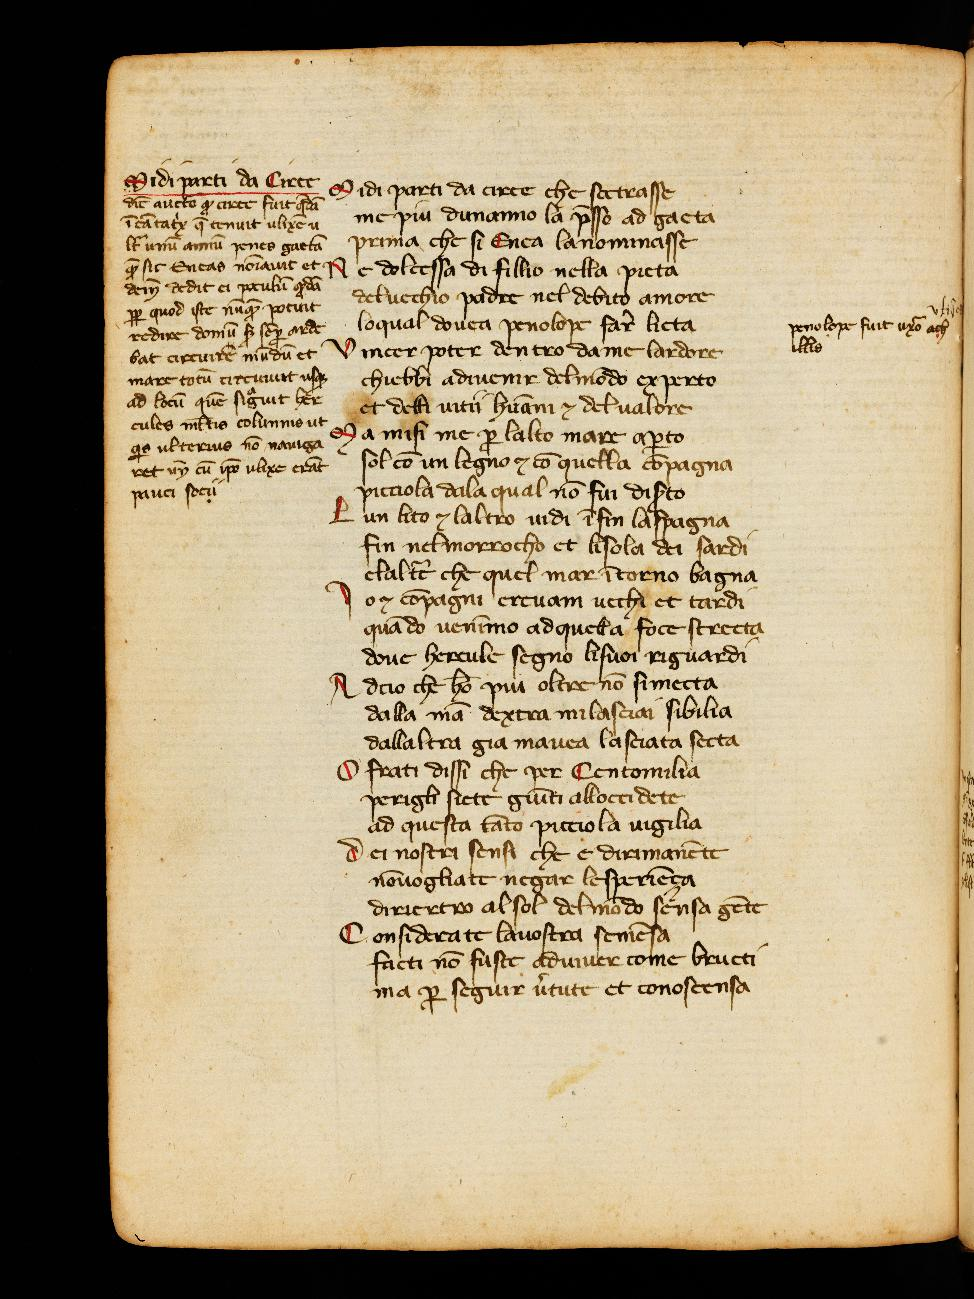
\includegraphics[height=4cm]{figures/datasets/HisDBSample0.jpeg}}
    &\raisebox{-.5\height}{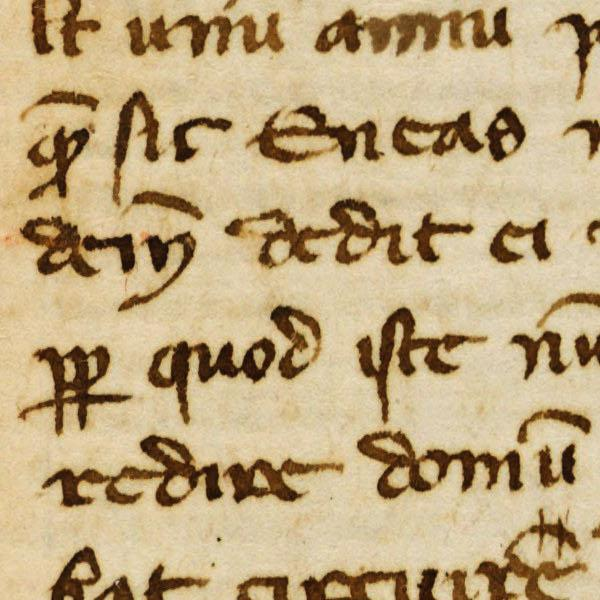
\includegraphics[height=4cm]{figures/datasets/HisDBSampleBox0.jpeg}}
     & \citefield{AlighieriColognyFondationMartin1300}{title}\\\vspace{0.5cm}  
     \raisebox{-.5\height}{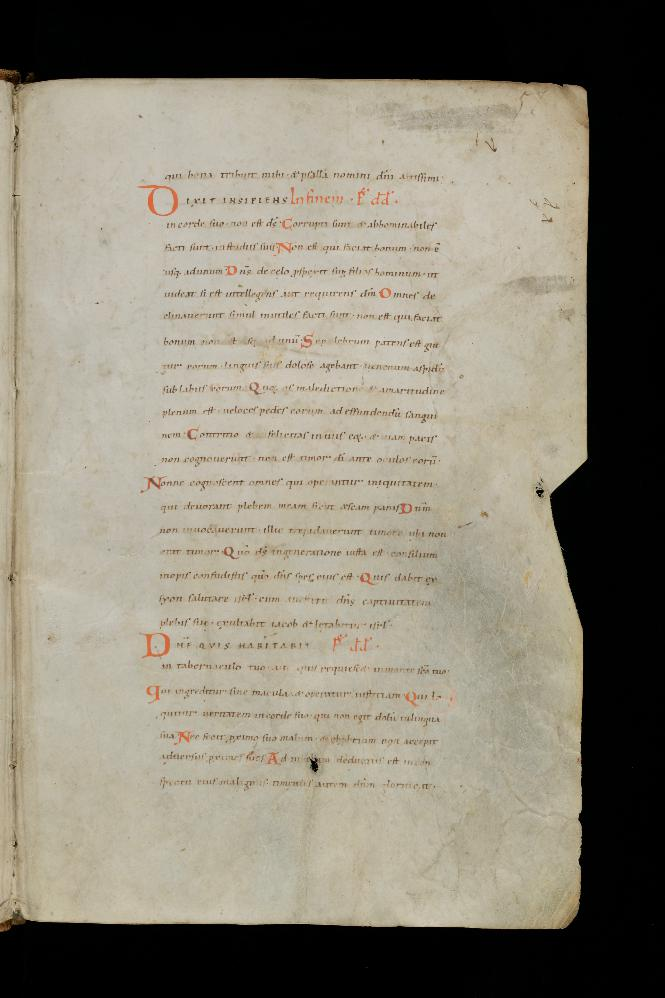
\includegraphics[height=4cm]{figures/datasets/HisDBSample1.jpeg}}
    &
    \raisebox{-.5\height}{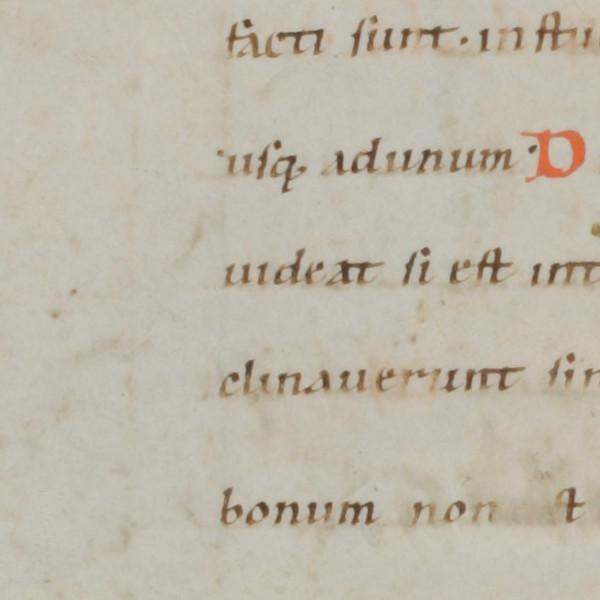
\includegraphics[height=4cm]{figures/datasets/HisDBSampleBox1.jpeg}}
     & \citefield{LucanusStGallenStiftsbibliothek1025}{title}\\\vspace{0.5cm} 
     \raisebox{-.5\height}{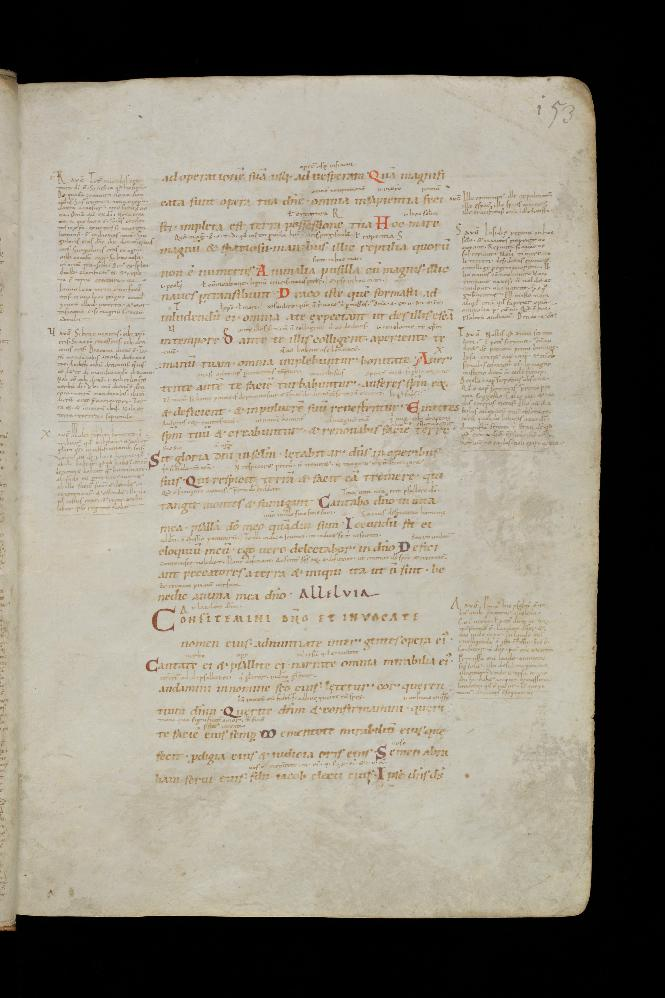
\includegraphics[height=4cm]{figures/datasets/HisDBSample2.jpeg}}
    &
    \raisebox{-.5\height}{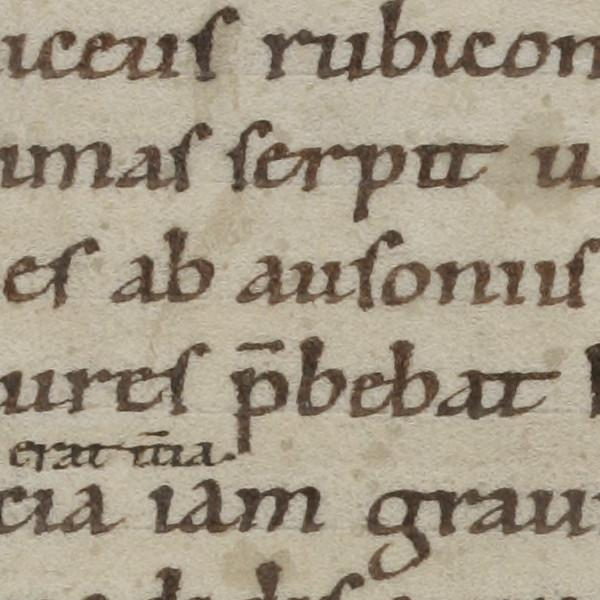
\includegraphics[height=4cm]{figures/datasets/HisDBSampleBox2.jpeg}}
     & \citefield{AmbrosiusStGallenStiftsbibliothek985}{title}\\\vspace{0.5cm}
    \end{tabular}
    \caption{HisDB Beipsiele mit Detailauschnitt}
\end{table*}
Die Manuskripte haben ein komplexes Layout und enthalten neben dem Haupttext auch Kommentare und Text-Dekorationen.
Die Manuskripte wurden mit einer Auflösung von 600 dpi gescannt und sind im  JPEG-Format gespeichert. 
Der Datensatz wurde manuell auf Pixelebene mit 4 Klassen annotiert (Hintergrund, Haupttext, Kommentar, Dekoration). Diese Ground-Truth-Annotationen sind im PAGE-XML-Format und als ``pixel-label'' PNG-Bilder gespeichert.


\begin{table*}
    \caption{Aufteilung der Seiten des DIVA-HisDB-Datenssets}

    \begin{tabular}{lccccc}
        {\bfseries Name} & {\bfseries Auflösung} & {\bfseries Training} & {\bfseries Validierung} & {\bfseries Test} & {\bfseries Test (ICDAR 2017)}\\
        \csvreader[head to column names]{tables/diva_hisdb_specs.csv}{}%
        {\name&	\width \(\times\)\height & \train	&\validate	&\test	&\comp\\}
    \end{tabular}
\end{table*}



%-------------------------------------------------------------------------------
\chapter{Reproduktion bisheriger Ergebnisse}
\label{chap:reproduktion}
\epigraph{What I cannot create, I do not understand}{--- Richarch Feyman}


Das erste Experiment basiert auf dem neusten Paper von \citeauthor{ChenConvolutionalNeuralNetworks2017}. 

\section{\textcite{ChenConvolutionalNeuralNetworks2017}}

\subsection{Vorverarbeitung}
\citeauthor{ChenConvolutionalNeuralNetworks2017} nutzen den Superpixelalgorithmus SLIC (simple linerar iterative clustering)
\cite{AchantaSLICSuperpixels2010} um die Dokumentenseiten in Superpixel einzuteilen.
Ein CNN klassifiziert dann Superpixel statt jeden Pixel einzeln.
Während des Trainings wird das Ground-truth Label des Zentrumpixels als Label für den Superpixel verwendet.

\citeauthor{ChenConvolutionalNeuralNetworks2017} verweisen für die Details zur Vorverarbeitung 
auf ihr Paper \cite{ChenPageSegmentationHistorical2016}. 
In diesem Paper werden die Bilder vor Anwendung des SLIC-Algorithmus mit einem Faktor von \(2^{-3}\)) skaliert.



\section{Bildverarbeitung mittels Neuronaler Netzwerke}
\section{CNN}
\section{SLIC Superpixel}
\cite{AchantaSLICSuperpixels2010}


\subsection{PyTorch}
% Genauer klären
PyTorch ist ein Framework zur automatischen Differenzierung von skaler Funktion \autocite{PaszkeAutomaticdifferentiationPyTorch2017}.

\section{Dokumentensegmetierung mittels CNN}



\section{\textcite{XuPageSegmentationHistorical2017}}
\section{VGG}
\section{Deconvolution}
\section{Ergebnisse}

%-------------------------------------------------------------------------------
\chapter{Selbstüberwachtes Lernen}
\label{chap:selfsupervised}

Jigsaw
\cite{NorooziUnsupervisedLearningVisual2016}
% \begin{figure}
%     \includegraphics[]{figures/graphs/exp.pdf} 
%     \caption{Image}
%   \end{figure}
%-------------------------------------------------------------------------------
\chapter{Umsetzung}

\section{Evaluierung}

\sfigure{Beispiel aus dem DIBCO2013-Dateset}{figures/tasks/DIBCO2013-dataset.pdf}

\subsection{Metriken}
Die Evaluierung der Ergebnisse der Segmentierung erfolgt auf Pixelebene.
\cite{LongFullyconvolutionalnetworks2015} berechnet 4 Metriken.
Sei \(n_{ij}\) die Anzahl der Pixel der Klasse \(i\) die der Klasse \(j\) zugeordnet wurden.


\newcommand{\resulttable}[3]{
    \begin{tabular}{l|r|r|r|r|r}%
    \hline
        \csvreader[head to column names, filter equal={\dataset}{#2}]{#1}{}%
        {#3}
        \end{tabular}
}
\begin{table*}
    \resulttable{results/document_image_segmentation_results.csv}{CB55}{ \name & \pixelacc & \FgPA & \meanacc & \meanIU & \fwIU\\}
    \resulttable{results/document_image_segmentation_results.csv}{CSG18}{  \pixelacc & \FgPA & \meanacc & \meanIU & \fwIU\\}
    \resulttable{results/document_image_segmentation_results.csv}{CSG863}{  \pixelacc & \FgPA & \meanacc & \meanIU & \fwIU\\}
        
\end{table*}

